\section{Discussion sur les choix opérés}

Du début jusqu'à la fin du projet, nous avons dû faire des choix de conduite. Nous recenserons dans cette partie les principales questions que nous nous sommes posées sur la marche à suivre.

\subsection{Environnement logiciel}

Comme il nous avait été conseillé de faire, nous nous sommes rapidement accordés sur l'environnement logiciel à adopter.
\begin{itemize}
 \item Utilisation de QtCreator, environnement de développement C++ open-source, multi-plateformes, et régulièrement mis à jour
 \item Développement sur Linux. Le choix n'était pas évident, étant donné que ce système d'exploitation ne faisait pas partie des cibles officielles du projet. L'intérêt était en fait de ne pas favoriser le développement sur Windows, avant de nous rendre compte que certains de nos choix avaient été faits au détriment de Mac OS X, ou inversement.

 Néanmoins, dès que la compilation a été possible de manière native sur Windows, un des membres du groupe est resté dessus
 pour le développement, ce qui a permis d'empêcher que des problèmes de compatibilité ne se propagent trop longtemps.

 De même, le programme était réguilèrement construit sous Mac OS X pour vérifier que la compatibilité n'était pas brisée par une manipulation malencontreuse.
 \item Utilisation du gestionnaire de version Git, et non de Subversion. La raison est que Git est de plus en plus utilisé, au détriment de SVN, et que le PFA était une excellente occasion pour apprendre à l'utiliser.
 \item Création du dépôt sur GitHub. Nous avons éliminé le dépôt de l'ENSEIRB-MATMECA en raison d'une coupure qui aura duré plusieurs jours en Octobre (en plus des fréquentes interruptions de ce service dont nous avions pris l'habitude au cours de l'année précédente), ainsi que de nombreux autres services tels que Sourceforge ou Google Code, car ceux-ci imposaient l'utilisation d'une licence libre (ce qui, a priori, n'est pas le cas de GuitarTutor) aux projets hébergés sur leur plate-forme, à moins de payer un abonnement mensuel. GitHub était également dans ce cas, mais une offre réservée aux étudiants nous a permis de bénéficier gratuitement d'un compte premium pour créer librement un dépôt privé, sans contrainte de licence.
\end{itemize}

Les différents choix énumérés ci-dessus ont été faits au début du projet en analysant les opinions de chacun, puis \textit{``officialisées''} en les listant sur notre wiki.


\subsection{Utilisation de Qt}

Le choix d'utiliser la librairie Qt s'est fait très rapidement, tant les avantages étaient évidents:
\begin{itemize}
 \item Le code source existant utilisait déjà Qt.
 \item Qt est utilisable aussi bien sur Mac OS X que sur Windows, ainsi que sur Linux.
 \item Le support officiel d'Android et iOS, les systèmes d'exploitation mobiles dominants sera effectif d'ici deux sous-versions de Qt,
 ce qui fait que le programme pourra être porté sans heurt sur tablette, smartphone... Il sera juste nécessaire d'ajuster les vues pour
 ces nouvelles plateformes.
 \item Le développement avec Qt est facilité par l'IDE que nous avons choisi, à savoir QtCreator.
 \item La documentation est très claire et complète.
 \item Qt est open-source et bénéficie d'une large communauté d'utilisateurs.
 \item Qt est incroyablement complet: interface graphique, XML, multimédia, socket, affichage de pages web\dots
 \item Plusieurs d'entre-nous avaient déjà des connaissances sur cette librairie.
\end{itemize}

Nous avons donc choisi d'adopter cette librairie dès les débuts du projet.

\subsection{Utilisation de FMOD}

FMOD est la librairie audio qui est utilisée aujourd'hui dans l'éditeur et dans le lecteur. Là encore, c'était cette même librairie qui servait déjà dans l'ancienne version de l'éditeur, dans la partie qui traitait les fichiers audio. En revanche, dans le lecteur, nous avons substitué la librairie \textit{libsndfile} pour FMOD.

FMOD comporte de nombreux avantages, comme par exemple la lecture de formats compressés tels que le MP3, aujourd'hui incontournable, mais aussi bien d'autres formats propriétaires courants, comme le WMA'.
Jusqu'à présent, \textit{libsndfile} limitait l'utilisation de GuitarTutor aux fichiers wav, ce qui contraignait l'utilisateur à manipuler des fichiers de très grande taille dans des formats non-compressés ou bien relevant de l'antiquité informatique comme Amiga, Atari\dots FMOD disposait également des mêmes fonctionnalités que celles qui étaient alors utilisées dans le code avec \textit{libsndfile}, ce qui permettait de ne pas géner la transition. FMOD nous a donc semblé être un bon choix, malgré le fait qu'il s'agisse d'une librairie propriétaire (nous n'avons pas eu de contre-indication de la part des clients à ce propos).
De plus, c'est un standard dans le monde des jeux vidéos, ce qui est une bonne formation pour ceux d'entre nous souhaitant partir dans ce domaine.


\subsection{Format d'échange en XML}
\label{xml}

L'échange entre l'éditeur et le lecteur se fait par l'intermédiaire de fichiers. Ces fichiers sont créés et modifiés par l'éditeur, puis lus dans le lecteur. Initialement, le format qui était utilisé listait les différentes parties du morceau, ainsi que les accords devant être joués et le temps en millisecondes correspondant (par rapport au début de la musique). Le fichier audio lu simultanément était, quant à lui, codé en dur dans le code source. Bien qu'il eût été facile de se contenter d'intégrer le chemin du fichier audio en début de fichier, nous avons préféré repenser totalement le format du fichier d'échange en nous basant sur le langage XML.

\begin{table}[H]
\begin{center}
\begin{tabular}{l|l}
 & \verb{<?xml version="1.0"?>{\\
 & \verb{<morceau timeSignature="4" line="16" chordMesure="1" end="261735"{ \\
 & \verb{  nom="Hotel California" comment="Un classique de 1976" column="4"{ \\
 & \verb{  fichier="Tracks/HotelCalifornia/EaglesHotelCalifornia.mp3"{ \\
 & \verb{  beginning="53145" bar="56402" artiste="The Eagles">{ \\
\verb{[COUPLET1]{ & \verb{  <partie nom="Couplet 1">{ \\
\verb{Bm 53145{ & \verb{    <accord nom="Bm" temps="53145" repetition="1"/>{ \\
\verb{F# 56402{ & \verb{    <accord nom="F#" temps="56402" repetition="1"/>{ \\
\verb{...{ & \verb{    ...{\\
 & \verb{  </partie>{\\
 & \verb{</morceau>{\\
\end{tabular}
\caption{Comparaison entre ancien et nouveau formats d'échange}
\label{fichiers_xml}
\end{center}
\end{table}

Nous avons demandé à M. Lombard, chargé de TD de XML et consultant pour Sopra Group, de nous conseiller sur la manière dont structurer notre document, et la proposition que nous lui avons faite (le format ci-dessus) lui a semblé cohérente par rapport à notre utilisation.

Comme on peut le voir sur l'exemple du tableau \ref{fichiers_xml}, notre format de fichier nous permet de contenir bien plus d'informations que l'ancien format. C'est un très gros avantage lorsqu'il s'agit notamment de recharger le fichier dans l'éditeur pour le modifier, puisque toutes les données qui ont été entrées lors de la création du fichier y ont été sauvegardées (même si certaines ne sont pas directement utilisées dans le lecteur).

Un second avantage est la facilité d'adaptation du format. En effet, si un jour il est décidé d'ajouter une nouvelle information dans le fichier XML, il n'y aura a priori pas besoin de modifier la façon de récupérer les informations. Cette maléabilité permise par le standard DOM (\textit{Document Object Model}) qui permet de naviguer au sein d'un document XML sans avoir à connaître tout son contenu. C'est justement la technique qui est mise en \oe uvre dans le module QtXML que nous avons utilisé (voir l'exemple de la figure \ref{xml_dom}).

\begin{figure}[H]
\begin{lstlisting}
//Récupération du premier accord de la partie courante
QDomNode chordNode = partElement.firstChild();
while(!chordNode.isNull())
{
  QDomElement chordElement = chordNode.toElement();

  //Récupération des informations de l'accord
  QString name = chordElement.attribute("nom", 0);
  int t = (chordElement.attribute("temps", 0)).toInt();
  int rep = (chordElement.attribute("repetition", 0)).toInt();

  //Création de l'objet représentant l'accord
  currentChord = new TrackChord(name, t, rep, previousChord, 0, currentPartTrack);
  //Ajout de cet accord à la liste des accords de la partie courante
  currentPartTrack->AddChord(currentChord);

  //Passage à l'accord suivant
  chordNode = chordNode.nextSibling();
}
\end{lstlisting}
\caption{Lecture d'un fichier XML, extrait de \texttt{TrackLoader::convertXmlToLogicalTrack}}
\label{xml_dom}
\end{figure}

\subsection{Reprise des bases précédentes}

Même s'il était au départ tentant de faire table rase et de recommencer le projet à zéro, tant la présentation du code existant laissait à désirer, nous avons fait l'effort de le remanier et de l'appréhender afin de pouvoir le réutiliser au maximum.

\subsubsection{Sur l'éditeur}

Nous avons gardé la base de l'interface de l'éditeur, à savoir le système de grilles, ainsi que le système d'arbre des accords. Nous avons ensuite ajouté peu à peu les différents éléments qui constituent aujourd'hui l'éditeur de grilles (voir figure \ref{av_ap_editeur}).

\begin{figure}[H]
\begin{center}
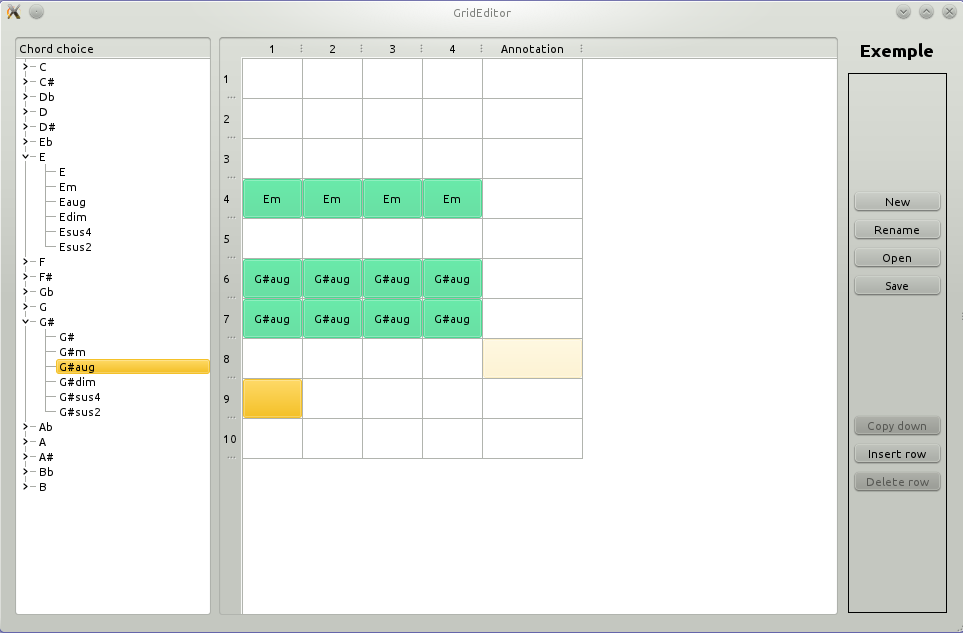
\includegraphics[width=225px]{ancien_editeur.png}
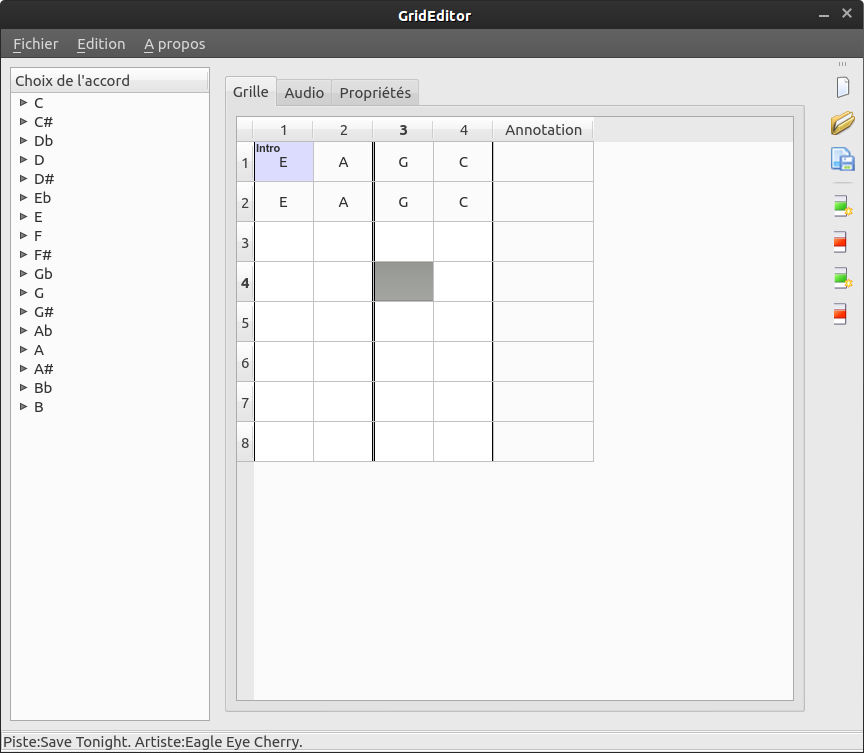
\includegraphics[width=225px]{nouveau_editeur.png}
\caption{L'éditeur de grilles, avant et après}
\label{av_ap_editeur}
\end{center}
\end{figure}


\subsubsection*{Quelques mots sur l'interface}

Un des points importants qui étaient à prendre en compte lors du développement était la nécessité de réaliser un logiciel accessible. L'expérience utilisateur était par conséquent un des facteurs clés. Le problème était que la tâche que l'utilisateur final doit réaliser avec le logiciel demandait un savoir-faire particulier (par exemple, synchroniser un tableau avec un morceau de musique), et il était donc primordial de la rendre le plus accessible possible, sans pour autant limiter les fonctionnalités.

Nous avons fait le choix de penser en premier lieu à l'expérience utilisateur, en créant une interface qui soit à la fois accessible et esthétique. Nous avons par exemple apporté:
\begin{itemize}
 \item la traduction en Français de l'interface
 \item la possibilité d'ajouter les accords au clavier, comme il serait tentant de faire, ainsi que le déplacement par tabulations
 \item une meilleure visibilité du découpage en mesures et en parties de la grille, et la possibilité de rentrer plusieurs accords par mesure
 \item une barre d'outils pour les actions les plus fréquentes, ainsi que des raccourcis claviers
 \item le rapprochement implicite entre la grille et le morceau (système d'onglets, et fusion des deux anciens éditeurs en un seul)
 \item la visualisation de l'information contenue dans le fichier audio
\end{itemize}

Le principal défi aura été de faciliter la synchronisation entre le morceau et la grille. Nous avons dans un premier temps mis en place un lecteur audio au sein de l'éditeur afin que l'utilisateur puisse aisément écouter le morceau qu'il est en train de créer. C'est ensuite qu'est venue l'idée, notamment à l'aide de nos clients, d'utiliser trois marqueurs temporels pour définir cette synchronisation:
\begin{enumerate}
 \item Un marqueur pour le début de la première mesure du morceau
 \item Un second marqueur pour signaler la fin de la première mesure
 \item Et un dernier pour signaler la fin du dernier accord du morceau
\end{enumerate}
Une fois les temps associés définis précisément, il est facile de définir le temps de début de chaque accord dans le morceau (voir l'algorithme sur la figure \ref{editor_time_caseitems}). Cette méthode nous a semblé particulièrement adaptée à notre situation, puisque les morceaux ciblés par l'application sont des morceaux qui sont rythmiquement très stables (c'est-à-dire que la durée de chaque mesure est supposée constante). De cette façon, l'utilisateur ne doit que très peu intervenir en comparaison avec l'ancienne méthode qui consistait à lui faire taper chaque temps du morceau.

Néanmoins, si nécessaire, l'utilisateur peut ajuster le temps mesure par mesure, et peut propager le changement sur une mesure à toutes
les mesures suivantes, comme dans le cas ou on rajouterai deux temps de pause entre un refrain et un couplet par exemple.

\begin{figure}[H]
\begin{lstlisting}
for (int r = 0 ; r < rmax ; r++) //Parcours des lignes
{
	for (int c = 0 ; c < cmax - 1 ; c ++) //Parcours des colonnes
	{
		QTime caseTime = MsecToTime(
				    (TimeToMsec(beginning) +
				      ((TimeToMsec(bar) - TimeToMsec(beginning))
				        /m_barsize)
				    * (r * (cmax - 1) + c)));
		((CaseItem*) item(r,c))->setBeginning(caseTime);
	}
}
\end{lstlisting}
\caption{Mise en place des temps de début des accords en fonction des marqueurs entrés par l'utilisateur, extrait de \texttt{ChordTableWidget::setTimeInfo}}
\label{editor_time_caseitems}
\end{figure}

La question était donc de trouver un moyen simple pour pouvoir indiquer de façon précise chacun de ces trois marqueurs temporels. Il nous est tout de suite venu à l'esprit d'utiliser les formes d'ondes du fichier audio désiré pour mieux cibler les débuts des accords. FMOD, pour les données spectrales, et Qt, pour l'interface, ont été très utiles pour l'implémentation. Un zoom et déplacement à la souris, inspiré de l'ergonomie des \ac{DAW} actuels, a également été mis en place sur cette même forme d'onde, ainsi que le positionnement des timers directement \textit{sur} la forme d'onde. Au final, le marquage devient une tâche relativement aisée et rapide (figure \ref{editor_audiosync}).

Enfin, dans le cas idéal ou le morceau aurait été joué au métronome, on peut directement rentrer le tempo dans l'éditeur.
\begin{figure}[H]
\begin{center}
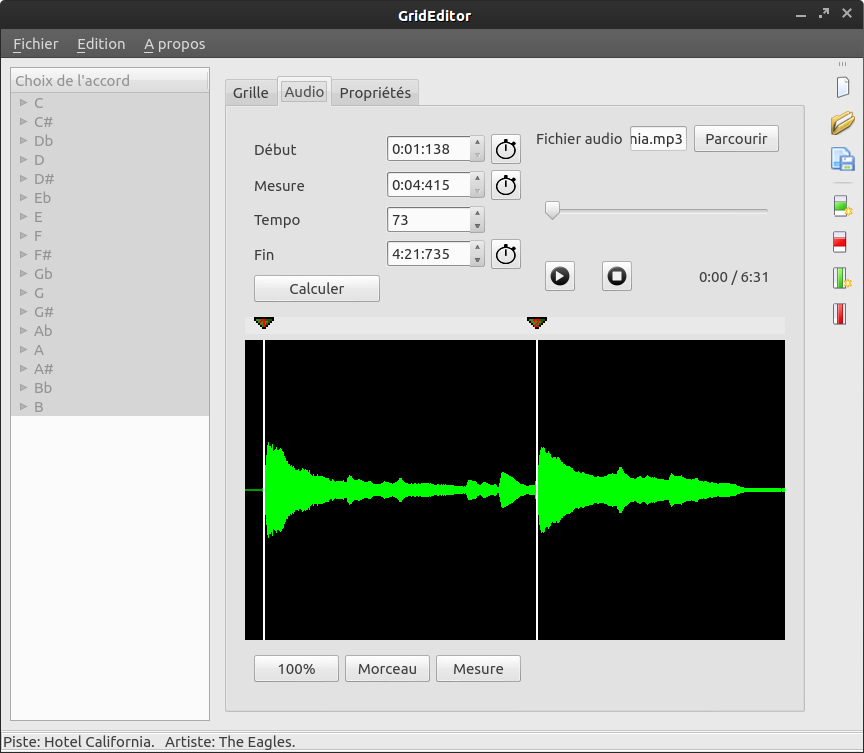
\includegraphics[width=400px]{editor_audiosync}
\caption{Synchronisation audio}
\label{editor_audiosync}
\end{center}
\end{figure}

\subsubsection{Sur le lecteur}

En ce qui concerne le lecteur, nous n'avons dans un premier temps que modifié l'interface. Celle-ci a été refaite intégralement selon la maquette qui avait été présentée en janvier (voir la figure \ref{annexe_proto_player} en annexe). Notre travail a finalement abouti à une interface semblable aux exigences qui avaient été fixées, certains détails ayant été revus en cours de développement en accord avec nos clients. L'objectif principal était de rendre le programme beaucoup plus convivial, mais aussi plus accessible. L'interface actuelle est présentée en figure \ref{interface_player}.

Dans un deuxième temps, nous avons fait le choix de revoir le fonctionnement interne du lecteur. Comme évoqué précédemment, nous avons ainsi commencé par faire disparaître la librairie \textit{IScoreLight}. En effet, celle-ci comportait plusieurs dizaines de fichiers sources (en pratique, 17000 lignes de code) qui, au final, n'étaient pas exploitées. De plus, le format que nous avons défini dans les classes \texttt{LogicalTrack}, \texttt{PartTrack} et \texttt{TrackChord} remplit exactement le besoin de positionnement dans le morceau que nous avions défini. La gestion de la navigation dans le morceau est donc confiée à la classe \texttt{SongManager} que nous avons créée.

Dans un deuxième temps, nous nous sommes attelés à remplacer la librairie \textit{libsndfile} par FMOD en vue de supporter de nouveaux formats audio. FMOD se charge en fait d'ouvrir le fichier audio demandé et de le mettre en mémoire. La gestion à proprement parler du son reste la tâche de PortAudio dans le lecteur.

Nous ne l'avons pas fait par manque de temps, mais l'idéal serait de remplacer aussi PortAudio par FMOD,
 ce qui peut se faire sans trop de problèmes car FMOD gère aussi les entrées audio.
 Cela permettrait de partager le code de lecture entre le lecteur et l'éditeur, ce qui n'est pas le cas actuellement.
 De plus, comme vu précédemment avec PortAudio, FMOD permet aussi de gérer les cartes sons ASIO, ce qui permettrait de basses
 latences pour l'entrée sous Windows.

Finalement, il ne reste aujourd'hui de la première version du lecteur que la gestion bas niveau du son, notamment l'analyse des accords effectuée par la librairie \textit{EHPCP}. Ce tri nous a permis d'améliorer grandement les performances, notamment lors de la compilation du programme (cf. figure \ref{refonte_code}).

\begin{figure}[H]
\begin{center}
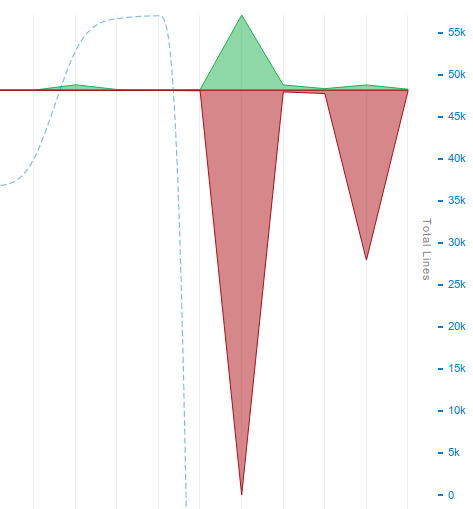
\includegraphics[width=300px]{refonte_code.png}
\caption{Suppression des bibliothèques Boost et IScoreLight du projet}
\label{refonte_code}
\end{center}
\end{figure}

Nous avons également fait en sorte que le lecteur utilise par défaut OpenGL, afin que celui-ci soit, au moins partiellement, exécuté sur la carte graphique de l'utilisateur, en vue d'améliorer là encore les performances. En effet, nous n'utilisons pas le système de widgets standard comme sur l'éditeur par exemple: nous avons utilisé le système de scène de Qt, qui permet plus de liberté graphique, ce que nous pensons adapté au monde ludique.
Ce système de scène est tout à fait représentatif de la \ac{MVC} : nous plaçons les éléments comme nous le désirons et Qt se charge
de la logique de mise à jour, de dessin, et de boucle centrale. Il suffit donc simplement de dire à Qt d'utiliser OpenGL via la ligne suivante :

\begin{figure}[H]
\begin{lstlisting}
setViewport(new QGLWidget);
\end{lstlisting}
\caption{Activation d'OpenGL dans le lecteur, extrait de \texttt{MyView::MyView}}
\label{player_opengl}
\end{figure}

et le dessin passe, lorsque c'est possible (c'est le cas sur tout ordinateur récent avec des pilotes graphiques à jour), par la carte graphique.

\subsection{Installateurs sur les différents systèmes d'exploitation}

Comme il nous avait été demandé, le programme devait être rendu sous la forme d'un installateur pour chacun des deux systèmes d'exploitation visés.

\subsubsection{Sur Windows}

Sur Windows, GuitarTutor se présente sous la forme d'un installateur \textit{msi} créé avec le logiciel Advance Installer. L'apparence de cet installateur est tout à fait semblable aux installateurs de logiciels Windows habituels, et propose les mêmes options; comme par exemple la possibilité de modifier le chemin de l'installation, ou encore celle de créer une icône sur le bureau de l'utilisateur.

La seule véritable difficulté sur ce système d'exploitation aura été de définir quelles étaient les librairies dynamiques à inclure dans notre package. Pour cela, nous avons testé sur des machines vierges de tout outil lié à notre environnement de travail (Qt, FMOD,\dots), puis simplement procédé par élimination pour ne retenir que les fichiers dll nécessaires.

Un outil qui a aussi été utilisé vers la fin du projet est Dependency Walker : ce programme analyse un fichier exécutable et liste les
DLL dont il a besoin.

\begin{figure}[H]
\begin{center}
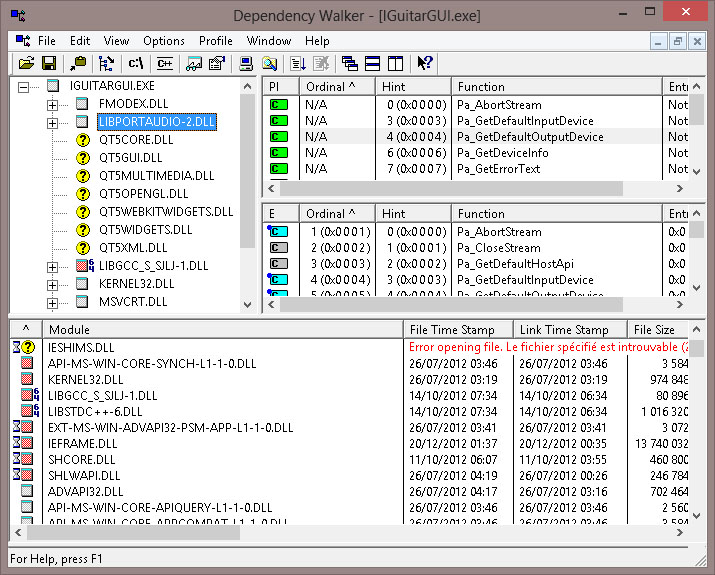
\includegraphics[width=300px]{depwalker.jpeg}
\caption{Dependency Walker}
\label{dep_walker}
\end{center}
\end{figure}

Nous avions un temps pensé à recompiler Qt de manière statique pour limiter la taille du programme ainsi que l'installation de DLL mais cela s'est révélé trop complexe à mettre en oeuvre.

\subsubsection{Sur Mac OS X}

Sur Mac OS X, notre programme se présente comme une application \textit{.app}, autrement appelé \textit{bundle}. C'est avec le format \textit{dmg}, sur ce système d'exploitation, une des deux formes les plus usuelles pour distribuer un logiciel. Il s'agit en fait d'un dossier contenant l'exécutable en lui-même, ainsi que tous les éléments tels que les bibliothèques dynamiques nécessaires à son fonctionnement (cf figure \ref{app_mac_os}).

\begin{figure}[H]
\begin{center}
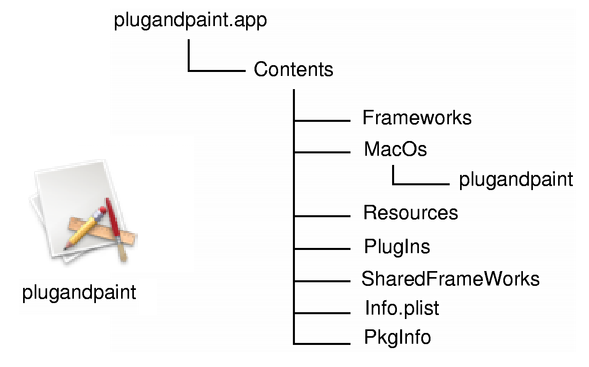
\includegraphics[width=300px]{bundle_mac.png}
\caption{Le bundle pour Mac OS X (d'après qt-project.org)}
\label{app_mac_os}
\end{center}
\end{figure}

Plusieurs outils similaires sont mis à la disposition des développeurs Mac OS X pour créer ces bundles. Nous avons, dans un premier temps, choisi d'utiliser l'utilitaire \textit{qtmacdeployment}, fourni avec Qt. Seulement, il s'est avéré que les bundles créés ne fonctionnaient pas sur toutes les machines en raison d'un problème concernant la bibliothèque dynamique de FMOD. Nous avons finalement opté pour un autre outil, du nom de \textit{install\_name\_tools}, fourni cette fois-ci avec l'environnement XCode, et qui a réglé notre problème de déploiement.

\subsection{Développement Agile}

En accord avec les conseils de notre responsable pédagogique, nous avons rapidement opté pour l'utilisation d'une méthode de développement de type agile. Le PFA état en effet une excellente occasion pour s'essayer à ce genre de méthodes qui sont de plus en plus employées dans des cadres professionnels.

\subsubsection{Réunions clients}

Dès le mois de novembre, nous avons mis en place un système de rendez-vous réguliers, généralement toutes les trois semaines avec nos clients. Ces réunions servaient tout d'abord à présenter le travail qui avait été effectué depuis le dernier rendez-vous, au travers d'une démonstration sur le logiciel en cours de développement. S'en suivait une discussion sur les différents points qui méritaient d'être relevés, afin de répartir les tâches en trois catégories: ce qui était fait et qui était validé, ce qui était fait mais restait à améliorer (ou à changer totalement), et enfin, ce qui restait à faire. Il ne restait alors qu'à fixer les objectifs à tenir d'ici le prochain rendez-vous.

Les avantages de travailler de la sorte se sont révélés au cours du projet. Tout d'abord, la possibilité de discuter de manière régulière de nos avancées avec nos clients était particulièrement intéressante, car cela permet d'instaurer un dialogue entre demandeurs et réalisateurs. On peut notamment remarquer que le cahier des charges (cf annexes) comporte plusieurs points qui n'ont pas été réalisés, ou qui ont été réalisés différemment de ce qui était initialement prévu, pas à cause d'un manque de temps, mais grâce à ce dialogue qui a permis d'affiner et de changer les besoins exprimés au fur et à mesure du développement du projet.

La figure \ref{agile} résume ce processus.

\begin{figure}[H]
\begin{center}
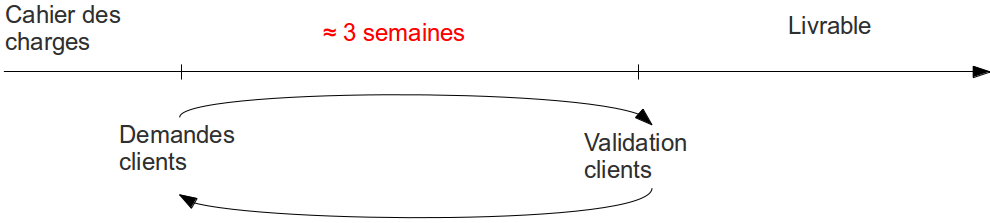
\includegraphics[width=450px]{methode_agile.png}
\caption{Schéma du processus de développement agile}
\label{agile}
\end{center}
\end{figure}

\subsubsection{Organisation de l'équipe et du travail}

De manière analogue au \textit{ScrumMaster} de la méthode Scrum, nous avons choisi au sein de notre équipe une personne en charge de veiller à la bonne application de notre méthode de développement. Sans se situer à un niveau supérieur aux autres, comme ce serait le cas pour un chef de projet, cette personne devait centraliser les travaux et les impressions de chacun pour aider à la répartition des tâches. Elle servait par ailleurs de \textit{représentant} de notre équipe pour nos clients et notre responsable pédagogique.

Les tâches étaient ensuite attribuées selon les demandes du cycle courant et des préférences de chacun, généralement par binômes, binômes qui ont été très variables tout au cours du projet. Des réunions hebdomadaires permettaient de faire le point sur les difficultés rencontrées et l'avancement des différentes tâches, et éventuellement de réorganiser la répartition. En plus de cela, l'équipe était informée par mail des interrogations et des avancées entre deux réunions, ainsi que par l'intermédiaire de notre wiki que nous avons mis en place dès le début du projet.

De manière générale, cette méthode de développement semble avoir bien fonctionné pour notre équipe au cours de ce projet.

\subsubsection{L'agile dans le code}
Un des autres aspects de l'approche agile au développement de projet est l'impact sur
la manière de produire du code. Notamment, comme cela a pu être vu au début du rapport dans la
chronologie du projet, il y a eu énormément de refactorisations et de changements assez profonds,
qui ont été annulés par la suite, comme pour BOOST, ou maintenus, comme pour FMOD.

\subsubsection{L'agile dans le cadre de l'école}
La difficulté principale avec le développement agile se situe dans les contraintes de temps
imposées par l'école et l'emploi du temps, dont les deux défauts sont d'être fixe (on ne peut pas ne pas aller en cours)
et variable (les horaires d'un même cours peuvent changer d'une semaine à l'autre).

De plus, notre répartition dans des groupes de TD différent a fait que nous n'avons pas toujours pu nous voir
comme nous le voulions, et que le gros du travail et des sprints était ainsi effectué généralement chez soi, en
communiquant par e-mail.

Ce qui aurait du être des post-its sur un tableau avec des tâches marquées dessus s'est retrouvé être un wiki
ou chacun pouvait barrer la tâche qu'il prenait en charge, néanmoins cette méthode est moins conviviale.

Le plus problématique dans cette approche est que la communication est plus difficile avec les autres
quand un binôme est bloqué, notamment.
